\chapter[EMF gränsvärden]{Elektromagnetiska gränsvärden}
\label{EMF}

\section{Inledning}
\index{elektromagnetiska fält (EMF)}
\index{EMF}
En amatörradiostation skickar ut radiovågor, signaler, för att kommunicera
trådlöst med hela världen.
Radiovågorna kallas även elektromagnetiska fält (EMF)
(eng. \emph{Electromagnetic Field (EMF)}).
Runt alla antenner som sänder ut radiovågor bildas elektromagnetiska fält av den
energi som skickas in i antennerna från radiosändaren.

Radiovågorna från en amatörradiostation, de elektromagnetiska fälten, klassas
som \emph{icke-joniserande strålning} och är som sådan strålning inte
tillräckligt energirik för att orsaka annat än uppvärmning av kroppens vävnad.

I allmänhet har studier visat att de nivåer av elektromagnetiska fält som
allmänheten kan utsättas för i närheten av en amatörradiostation ligger långt
under de värden där kroppstemperaturen skulle öka.

\index{icke-joniserande strålning}
\index{strålning!icke-joniserande}
Icke-joniserande strålning, som optisk strålning (infraröd strålning,
synligt~ljus och ultraviolett~strålning) och elektromagnetiska fält (radiovågor
och mikrovågor) är normalt inte lika energirik som joniserande strålning.
När elektromagnetisk strålning absorberas i biologisk vävnad eller material är
den dominerande effekten därför endast en temperaturhöjning i vävnaden eller
materialet.

\index{joniserande strålning}
\index{strålning!joniserande}
Joniserande strålning är partikelstrålning eller elektromagnetisk strålning som
har tillräcklig energi för att rycka loss elektroner från de atomer som den
träffar och förvandla dem till positivt laddade joner, jonisering.
Exempel på joniserande strålning är röntgenstrålning och strålning från
radioaktiva ämnen.
Energin hos joniserande strålning kan vara så hög att den kan tränga in i
kroppen och påverka cellstruktur samt arvsmassa (DNA) i biologiskt material.

\index{WHO}
\index{World Health Organization (WHO)}
\index{International Commission on Non-Ionizing Radiation Protection (ICNIRP)}
\index{ICNIRP}
Inom World Health Organization (WHO) finns ett program som kallas
''The International EMF Project'' och där samlas all vetenskaplig
information som finns om biologiska effekter orsakade av elektromagnetiska fält.
''International Commission on Non-Ionizing Radiation Protection'', (ICNIRP)
är en fristående organisation (erkänd av WHO) som bland annat använder denna
information för att utveckla riktlinjer för begränsning av exponeringsnivån för
elektromagnetiska fält.
Dessa riktlinjer används av många länder.

\index{Strålsäkerhetsmyndigheten (SSM)}
\index{SSM}
\index{International Commission on Non-Ionizing Radiation Protection (ICNIRP)}
\index{ICNIRP}
Strålsäkerhetsmyndigheten (SSM) är den myndighet som har det formella ansvaret
för strålskydd i Sverige.
Myndigheten ska bland annat förebygga akuta skador och minska risken för sena
hälsoeffekter hos allmänheten till följd av exponering för elektromagnetiska
fält.

SSM har tagit fram allmänna råd SSMFS 2008:18 \cite{SSMFS2008:18} för
begränsning av allmänhetens exponering för elektromagnetiska fält.
De allmänna råden anger vilka referensvärden som gäller i Sverige.
Råden utgår från rekommendationer i EU-direktiv 1999/519/EG \cite{1999/519/EG}.
EU-direktivet följer i sin tur de riktlinjer för begränsning av
elektromagnetiska fält som sammanställts av ICNIRP.

Eftersom grunden i amatörradioutövandet är att generera elektromagnetiska fält
för att kommunicera via radio så är kunskapen om EMF viktig.
Med de möjligheter radioamatörer har, måste de allmänna råden gällande EMF
följas.
Förståelsen för hur fält uppträder och hur de kan begränsas anses vara
fundamental kunskap för radioamatörer.

\section{Fält}
\index{elektriskt fält (E)}
\index{magnetiskt fält (H)}
För att ange nivån på det elektriska fältet (E) används enheten
''volt per meter'' (V/m).
Det magnetiska fältet (H) nivå anges i enheten ''ampere per meter'' (A/m).

Antennens uppgift är att så effektivt som möjligt omvandla den högfrekventa
strömmen i matarkabeln till en elektromagnetisk våg som utbreder sig i luften.

Den sammansatta elektromagnetiska vågen uppträder inte direkt vid antennen utan
uppstår i det som man kallar fjärrfältet.
Detta sker genom växelverkan mellan de elektriska och magnetiska fält som
utgår från antennen.

Teorierna som beskriver hur denna växelverkan fungerar är komplicerade
men det viktiga att förstå är att det finns en gräns mellan vad man
kallar fjärrfältet, längre bort från antennen och närfältet nära antennen.

\index{fjärrfält}
I fjärrfältet kan man på grund av växelverkan mellan det elektriska- och det
magnetiska fältet mäta vilket som helst av dem.
I och med att det elektromagnetiska fältet sprider ut sig över en större yta så
avtar styrkan i fältet med avståndet från antennen.
Det sammansatta elektromagnetiska fältet som passerat gränsen till fjärrfältet
avtar linjärt med avståndet, dubbleras avståndet halveras fältstyrkan.
Det spelar ingen roll om antennen är helt rundstrålande eller koncentrerar
effekten i en riktning, det elektromagnetiska fältet avtar på samma sätt.

\index{närfält}
I närfältet behöver man på grund av fältens komplicerade inbördes förhållande
mäta både det elektriska- och det magnetiska fältet för att få en uppfattning
om storleken på det radiofrekventa fältet.
I antennens närhet varierar nivåerna på de olika fälten kraftigt och på vissa
punkter kan höga fältstyrkenivåer mätas upp.

Om antennen har stor utsträckning i förhållande till använd våglängd kan ibland
fjärrfältsformler användas för att överslagsmässigt beräkna fältstyrkenivå i
antennens närfält.
För kompakta antenner (t.ex. små loopar) krävs komplicerade beräkningar
med hjälp av antennsimuleringsprogram.

Beroende på den antenntyp som genererar fältet är det antingen ett elektriskt
eller magnetiskt fält som dominerar i närfältet.
Elektrisk fältdominans genereras av antenntyper som bygger på
spänningsskillnader (t.ex. dipol) och magnetisk fältdominans av antenner
med strömflöde (t.ex. små loopar).

Eftersom alla elektriska ledare kan betraktas som antenner kommer dessa att
kunna generera fält, oavsett om det är tänkt att det ska vara en antenn eller
inte.
Man bör ha detta i åtanke vid installation av matarledning till antennen för
att undvika att högfrekvent ström flyter tillbaka till stationen på utsidan av
ledningen.
Även de apparater man använder för att generera radiosignaler kan ha dålig
skärmning och därigenom leds högfrekvent ström till apparaternas utsida.

Det finns alltså en risk att fältstyrkorna kan vara betydande i närheten av
sändare och framför allt vid slutsteg med tillhörande kablage.

\section{Allmänna råd}
\index{EMF!allmänna~råd}

SSM har gett ut allmänna råd för begränsning av allmänhetens exponering
för elektromagnetiska fält SSMFS~2008:18 \cite{SSMFS2008:18}.

Syftet med de allmänna råden är att skydda allmänheten från akuta
skadliga biologiska effekter vid exponering för elektromagnetiska fält.

I råden anges grundläggande begränsningar och härledda referensvärden.

\begin{quote}
	De grundläggande begränsningarna säkerställer att elektriska eller
	magnetiska fenomen som kan uppträda i kroppen inte stör funktioner i
	nervsystemet eller ger upphov till skadlig värmeutveckling.
\end{quote}

De grundläggande begränsningarna är, enligt internationella rekommendationer,
satta vid ungefär två procent av de nivåer vid vilka akuta biologiska effekter
är vetenskapligt säkerställda.

Från de grundläggande begränsningarna har härletts referensvärden som utgörs
av storheter som är mätbara utanför människokroppen.
Referensvärdena ska säkerställa att de grundläggande begränsningarna inte
överskrids.

\begin{quote}
	Om uppmätta värden överstiger referensvärdena, innebär detta inte nödvändigtvis
	att de grundläggande begränsningarna överskrids. I sådana fall gäller enligt
	dessa allmänna råd de grundläggande begränsningarna.
\end{quote}

I EU-direktivet 1999/519/EG \cite{1999/519/EG} skrivs att i sådana fall skall det
göras en bedömning huruvida exponeringsnivån ligger under den grundläggande
begränsningen.

Referensvärdena i de allmänna råden bör inte överskridas i något område där
allmänheten kan vistas under sådana tider att begränsningarna är av betydelse.

\index{EMF!akuta biologiska effekter}
Det finns två huvudsakliga akuta biologiska effekter som kan förekomma vid
kraftig exponering för elektromagnetiska fält.
Fält med frekvens upp till cirka 10~MHz kan om strömtätheten blir hög i kroppen
påverka det centrala nervsystemet.
Fält med frekvenser från 100~kHz till 10~GHz kan vid höga nivåer leda till en
uppvärmning av kroppen.

\index{Specific Absorption Rate (SAR)}
\index{SAR}
När elektromagnetisk strålning absorberas i biologisk vävnad kan vävnaden värmas
upp.
Detta benämns ''Specific Absorption Rate'' (SAR) som mäts i enheten watt per
kilogram (W/kg) eller milliwatt per gram (mW/g).
SAR definieras som den energi, medelvärdesbildad över hela kroppen eller delar
av kroppen som absorberas per tidsenhet och per massenhet biologisk vävnad.

Då uppvärmningen av kroppsvävnad inte går snabbt räknar man med den medeleffekt
som under en viss tid orsakar uppvärmning.
För frekvenser mellan 100~kHz och 10~GHz beräknas SAR-värdet som medelvärdet under
en sexminutersperiod.
För beräkning av SAR-värde på frekvenser överstigande 10~GHz hänvisas till
formler för beräkning enligt SSMFS 2008:18.

Beroende på kroppens storlek i förhållande till det elektromagnetiska fältets
riktning och våglängd skapas resonansfenomen på grund av att kroppen fungerar
som en antenn.
Detta påverkar uppvärmningen på så sätt att vid frekvenser som är nära kroppens
eller kroppsdelens elektriska resonansfrekvens absorberas effekten lättare och
maximal uppvärmning uppstår.
Hos vuxna ligger denna resonansfrekvens mellan 70- och 90~MHz om personen står
upp är och isolerad från något som kan jämföras med ett jordplan.
Även de olika kroppsdelarna kan vara resonanta.
En vuxen persons huvud är till exempel resonant vid cirka 400~MHz.

Kroppens storlek avgör alltså vid vilken frekvens den absorberar mest effekt och
vid frekvenser över och under resonansfrekvensen så minskar uppvärmningen
orsakad av det elektromagnetiska fältet.

\index{EMF!referensvärden}
Referensvärdena tar hänsyn till detta faktum och det mest restriktiva
frekvensområdet ligger inom området 10 till 400~MHz där effekt lättast
absorberas av kroppen.

I frekvensområdet 10 till 110~MHz finns även en begränsning till 45~mA för
inducerad ström i varje extremitet i syfte att begränsa det lokala SAR-värdet.

\begin{figure*}[htb]
	\begin{center}
		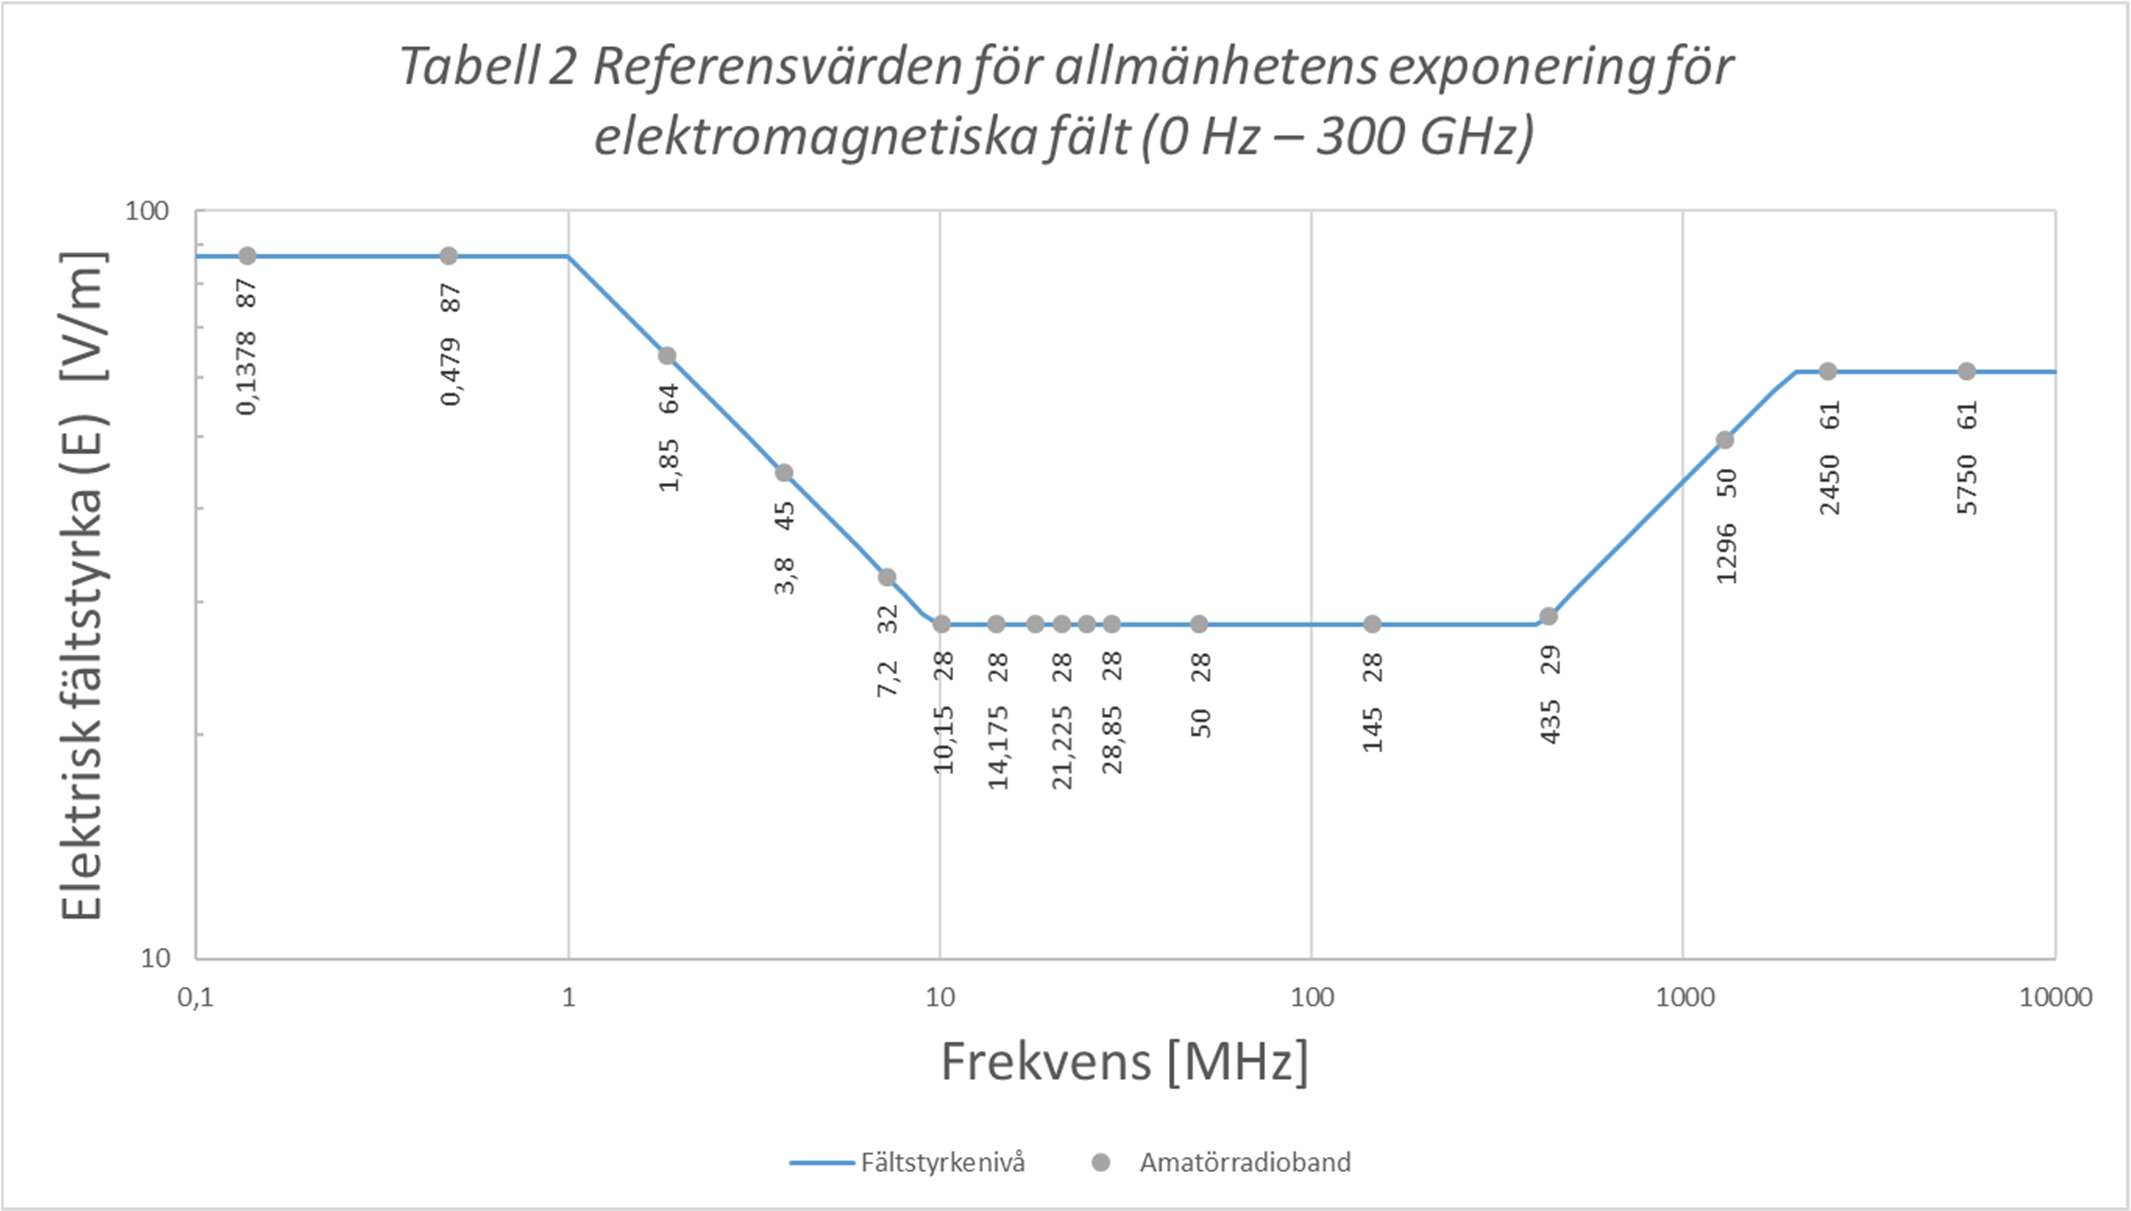
\includegraphics[width=13cm]{images/emfbild-000}
		\caption{Referensvärden för begränsning av elektriska fält (100~kHz--10~GHz)}
		\label{fig:emf1}
	\end{center}
\end{figure*}

Bild \ref{fig:emf1} illustrerar referensvärden för begränsning av elektriska
fält på platser där allmänheten kan vistas (100~kHz--10~GHz), med amatörband
och fältstyrkenivå angivna, till exempel 10,15~MHz har en högsta tillåtna
elektriskt fältstyrka på 28~V/m.

\begin{figure*}[htb]
	\begin{center}
		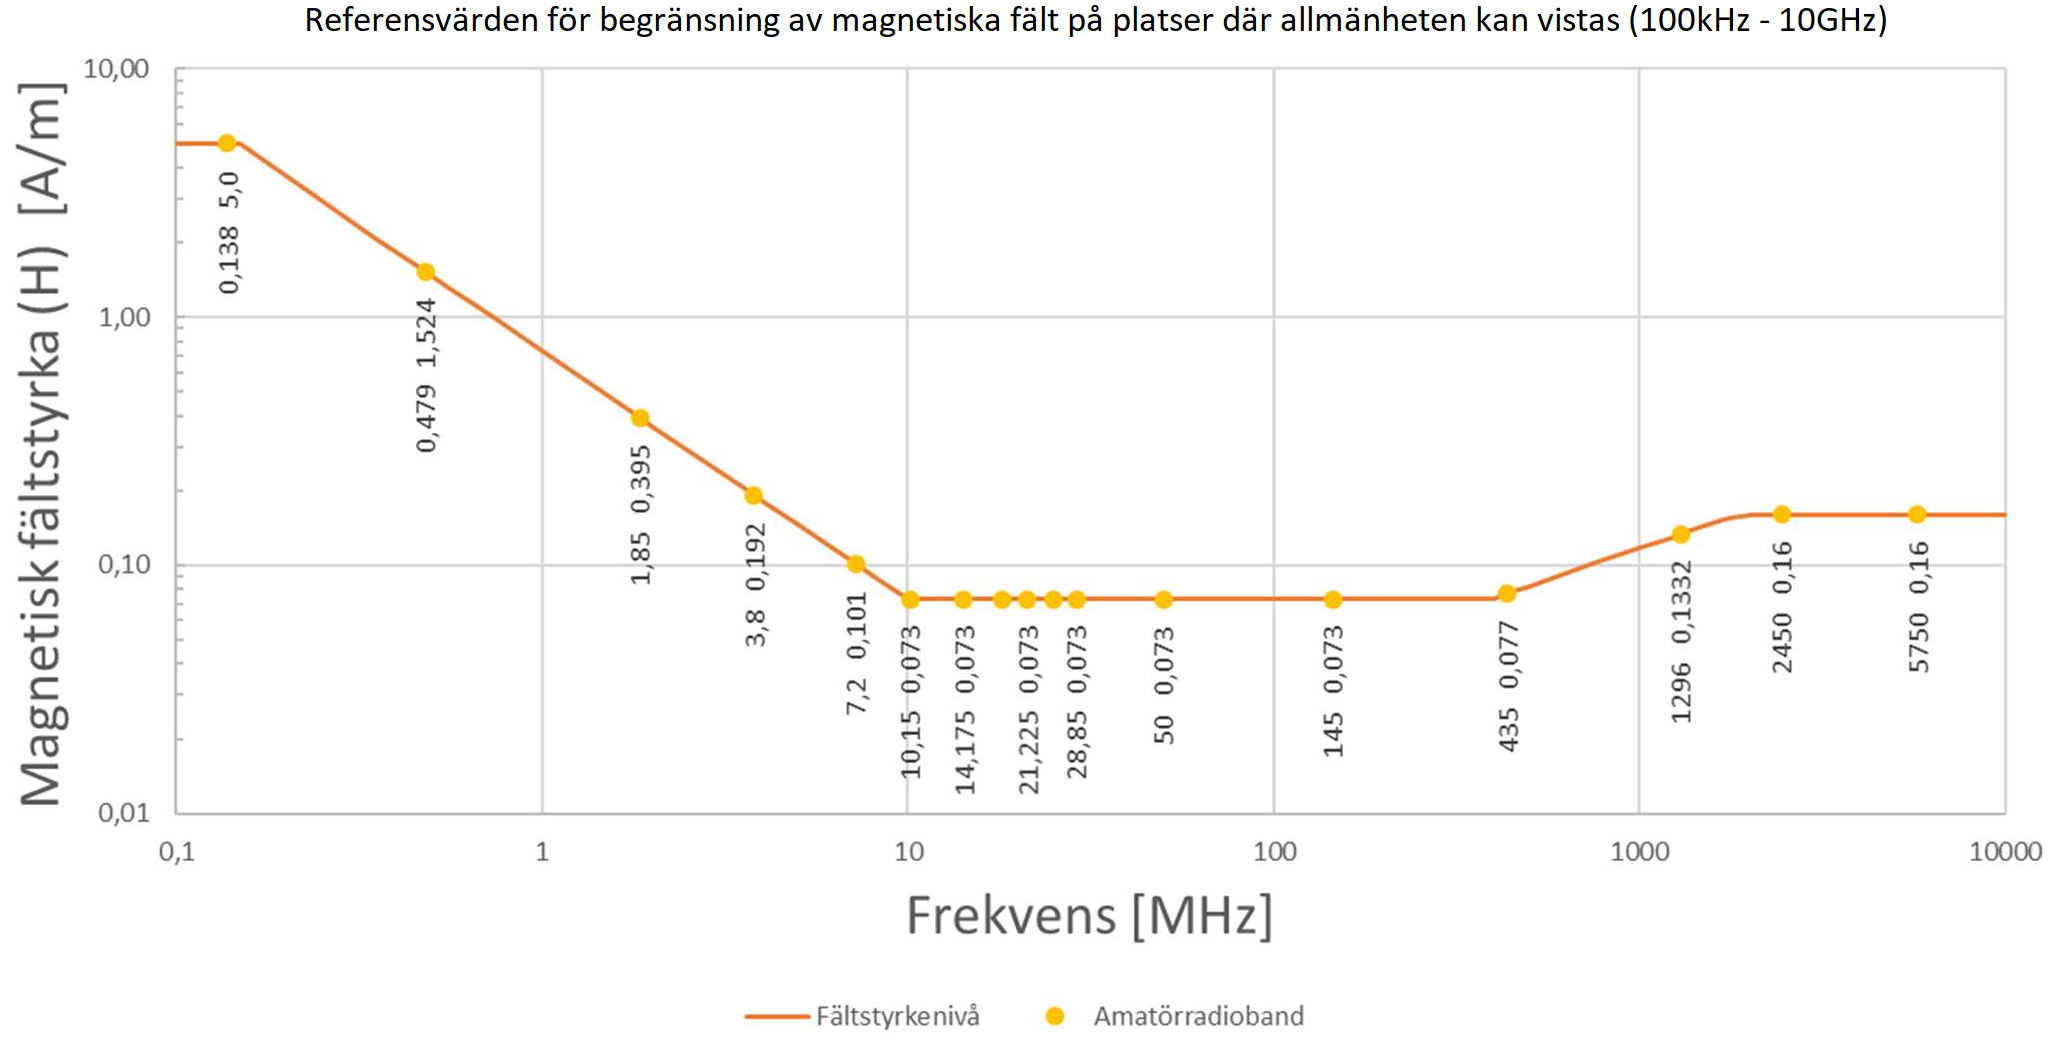
\includegraphics[width=13cm]{images/emfbild-001}
		\caption{Referensvärden för begränsning av magnetiska fält (100~kHz--10~GHz)}
		\label{fig:emf2}
	\end{center}
\end{figure*}

Bild \ref{fig:emf2} illustrerar referensvärden för begränsning av magnetiska
fält på platser där allmänheten kan vistas (100~kHz--10~GHz), med amatörband
och fältstyrkenivå angivna, till exempel 10,15~MHz har en högsta tillåtna
magnetisk fältstyrka på 73~mA/m.

\section{Utvärdering av EMF}
\index{EMF!utvärdering}

För att kunna utvärdera att den egna radiostationen vid sändning ger
elektromagnetiska fält som understiger referensvärdena behöver man känna till
de parametrar som är avgörande för styrkan på det elektromagnetiska fältet.
\begin{itemize}
	\item antennens förstärkning (G)
	\item sändningens medeleffekt (P)
	\item transmissionsledningens förluster (k)
	\item distansen (d)
\end{itemize}

\subsection{Antennen}
Antennen tar emot signalen från sändaren via en matningskabel och
omvandlar denna signal till en elektromagnetisk våg.
Hur effektivt antennen omvandlar signalen från sändaren kan enklast förklaras
med begreppen förstärkning eller antennvinst.

Man måste alltså känna till vilken förstärkning antennen har uttryckt i linjära
faktorer i förhållande till en isotrop antenn.

Antennförstärkning i förhållande till en isotrop antenn uttrycks vanligen i dBi.
Detta medför att en vanlig dipolantenn som används som referens för 0~dBd har
en förstärkning på 2,15~dBi jämfört med en isotrop antenn.

Alla värden på antennförstärkning uttryckt i dBd ska därför ökas med 2,15 för
att kunna användas i nedanstående tabell som visar förhållandet mellan
förstärkning i dB och linjära faktorer.

\begin{tabular}{|l|ccccccccccc|}
	\hline
	dB     &  0  &  1  &  2 & 2,15 &  3  &  4  &  5  &  6  &  7  &  8  &  9  \\ \hline
	G & 1,0 & 1,3 & 1,6 & 1,64 & 2,0 & 2,5 & 3,2 & 4,0 & 5,0 & 6,3 & 7,9 \\ \hline
	dB     &  10  &  11  &  12  &  13  &  14  &  15  &  16  &  17  &  18  &  19  &  20 \\ \hline
	G & 10,0 & 12,6 & 15,8 & 20,0 & 25,1 & 31,6 & 39,8 & 50,1 & 63,1 & 79,4 & 100,0 \\ \hline
\end{tabular}

För en antenn med förstärkningen 7~dBi ska alltså värdet 5,0 användas.

\textbf{G = Antennens förstärkning i linjära faktorer}

\subsection{Sändareffekten}
Alla SAR-värden ska beräknas som ett medelvärde under en period av sex minuter.
För att kunna utföra en beräkning av effektens medelvärde behövs utöver
PEP-effekt kännedom om de två faktorer som påverkar medeleffekten.
Faktorerna har därför betydelse för nivån på det elektromagnetiska fältet och
påverkar därigenom den genomsnittliga exponeringen för EMF.

\subsubsection{Modulationsfaktor:}
\index{EMF!modulationsfaktor}
\index{modulationsfaktor}

Beroende på trafiksätt så blir medeleffekten olika.
Används FM så medför det modulationssättet att man använder max uteffekt
kontinuerligt jämfört med SSB där medeleffekten beror på hur man talar.

Nedanstående tabell är de faktorer som enligt OET bulletin 65 supplement b,
\cite{OETbul65b} används i USA för att räkna ut medeleffekten på grund
av modulationsfaktorn.

\begin{tabular}{|l|c|}
	\hline
	Trafiksätt & Modulationsfaktor \\ \hline
	SSB & 0,2 \\ \hline
	CW & 0,4 \\ \hline
	SSB med processing & 0,5 \\ \hline
	FM & 1,0 \\ \hline
	MGM (t.ex. RTTY,PSK) & 1,0 \\ \hline
	Bärvåg & 1,0 \\ \hline
\end{tabular}

\subsubsection{Intermittensfaktor:}
\index{EMF!intermittensfaktor}
\index{intermittensfaktor}

Vid vanlig amatörradioanvändning sänder man inte kontinuerligt då växling
mellan sändning och lyssning sker regelbundet.
Sänder man och tar emot lika mycket under en sexminutersperiod så blir faktorn
0,5 men om man lyssnar mycket mer och sänder sällan blir faktorn mindre.

\begin{tabular}{|c|c|c|}
	\hline
	Sändning  & Mottagning & Intermittensfaktor \\
	(minuter) & (minuter)  & \\ \hline
	1 & 5 & 0,17 \\ \hline
	2 & 4 & 0,33 \\ \hline
	3 & 3 & 0,50 \\ \hline
	4 & 2 & 0,67 \\ \hline
	5 & 1 & 0,83 \\ \hline
	6 & 0 & 1,00 \\ \hline
\end{tabular}

\subsubsection{Medeleffekt:}
\index{EMF!medeleffekt}

För att räkna ut vilken medeleffekt som används ska man ta hänsyn
till både modulationsfaktor och intermittensfaktor enligt följande

\(Medeleffekt = Maxeffekten \cdot Modulationsfaktor \cdot Intermittensfaktor\)

\textbf{P = Medeleffekten under en sexminutersperiod}

\subsection{Kabeldämpning}
\index{EMF!kabeldämpning}

När uteffekten mäts vid sändaren och fältet genereras av effekten som
når antennen måste även den dämpning som matarledaren har vara känd.
Annars överskattas den genererade fältstyrkan.

Även här måste linjära faktorer användas.
Förlusterna i en kabel har negativa värden uttryckt i dB vilket medför att
faktorerna i nedanstående tabell blir mindre än ett.

\begin{tabular}{|l|c|c|c|c|c|c|c|c|c|c|c|}
	\hline
	dB & 0,0  & 0,5  & 1,0  & 1,5  & 2,0  & 2,5  & 3,0  & 3,5  & 4,0  & 4,5  & 5,0 \\ \hline
	k  & 1,00 & 0,89 & 0,79 & 0,71 & 0,63 & 0,56 & 0,50 & 0,45 & 0,40 & 0,35 & 0,32 \\ \hline
\end{tabular}

För en kabel med dämpningen 2,5~dB ska alltså värdet 0,56 användas.

\textbf{k = Matarkabels dämpning i linjära termer}

\subsection{Distans}
\index{EMF!distans}

För att kunna beräkna nivån på det elektromagnetiska fältet på en utvald plats
behöver man veta distansen till den sändande antennen.

Enligt Strålsäkerhetsmyndighetens allmänna råd så bör inte referensvärdena
överskridas på platser där allmänheten vistas.
En bedömning bör därför göras över distanserna från den sändande antennen till
platser allmänheten riskerar att exponeras för elektromagnetiska fält.

\textbf{d = Distansen från antennen till platsen där fältstyrkan ska bestämmas}

\subsection{Beräkning}
\index{EMF!beräkning}

Beräkning av det elektromagnetiska fältet kan med enkelhet bara
genomföras i fjärrfältet från en antenn.
I fjärrfältet vet vi sedan tidigare att man antigen kan utvärdera det
elektriska eller det magnetiska fältet.
Av denna anledning beskrivs här enbart beräkning av det elektriska fältets del av
det elektromagnetiska fältet.

Ett vedertaget avstånd från antennen där fjärrfältsberäkningar kan genomföras
är \(d=\dfrac{\lambda}{6}\).

Följande formler gäller enbart för beräkning av korrekt fältstyrka i
fjärrfältet men kan för enklare antenner användas för att uppskatta den
fältstyrka som uppträder i närfältet.

\begin{tabular}{|l|c|c|c|c|c|c|c|c|c|c|}
	\hline
	Band [m] & 160 & 80 & 40 & 30 & 20 & 17 & 15 & 12 & 10 & 6 \\ \hline
	Fjärrfältsgräns [m] & 27 & 13 & 6,7 & 5 & 3,3 & 2,8 & 2,5 & 2 & 1,7 & 1 \\ \hline
\end{tabular}

\textbf{E = Det elektromagnetiska fältets storlek i fjärrfältet}

Det elektromagnetiska fältets storlek (i fjärrfältet) räknas ut från
effekten (medelvärde), antennförstärkningen, matarledningens dämpning
och avståndet enligt följande förenklade formel.

\(E=\dfrac{\sqrt{30 \cdot P \cdot G \cdot k}}{d}\)

Genom enkel matematik kan man då använda samma formel för att räkna
ut på vilket avstånd man genererar en viss fältstyrka.

\(d=\dfrac{\sqrt{30 \cdot P \cdot G \cdot k}}{E}\)

Denna beräkning är enbart relevant för huvudloben.
Fältet under antennen beräknas inte, och därför kan resultatet inte användas
för att bedöma höjd på eller säkerhetsavstånd till antenntorn.
Använd dataprogram för att få bra bedömning på hur en antenn beter sig,
särskilt med avseende på antenner med riktverkan.

\subsubsection{Exempel 1:}

Vilken medelfältstyrka genererar man på ett visst avstånd från antennen?

En riktantenn för 144~MHz med förstärkning enligt databladet på
14,92~dBi (31 gånger).
Max uteffekt är 1000~W och trafiksättet är MGM (t.ex. RTTY, PSK) med
30 sekunders intervaller.
Den valda matarledningen har en dämpning på 2,5~dB (0,56~gånger).
Avståndet från antennen till beräkningspunkten är 15~m.

\(P_{medel} = P_{pep} \cdot modulationsfaktor \cdot intermittensfaktorn
= 1000 \cdot 1 \cdot 0,5 = 500\ \mathrm{W}\)

\(G = 31 \quad k = 0,56 \quad d = 15\)

\(E = \dfrac{\sqrt{30 \cdot P \cdot G \cdot k}}{d}
= \dfrac{\sqrt{30 \cdot 500 \cdot 31 \cdot 0,56}}{15}
= 34,02\ \mathrm{V/m}\)

Då referensvärdet på denna frekvens är 28~V/m, överskrider
amatörradiosändningen referensvärdet på detta avstånd.

\subsubsection{Exempel 2:}

På vilket avstånd från antennen når man referensvärdet?

En riktantenn för 144~MHz med förstärkning enligt databladet på
14,92~dBi (31 gånger).
Max uteffekt är 1000~W och trafiksättet är MGM (t.ex. RTTY, PSK) med
30~sekunders intervaller.
Den valda matarledningen har en dämpning på 2,5~dB (0,56~gånger).
Referensvärdet för 144~MHz är 28~V/m.

\(P_{medel} = P_{pep} \cdot modulationsfaktor \cdot intermittensfaktorn
= 1000 \cdot 1 \cdot 0,5 = 500\ \mathrm{W}\)

\(G = 31 \quad k = 0,56 \quad E = 28\)

\(d = \dfrac{\sqrt{30 \cdot P \cdot G \cdot k}}{d}
= \dfrac{\sqrt{30 \cdot 500 \cdot 31 \cdot 0,56}}{28}
= 18,22\ \mathrm{m}\)

För att följa de allmänna råden bör allmänheten inte kunna vistas i huvudloben
framför antennen på ett avstånd mindre än 19~m då sändning utförs enligt
exemplet.

\subsubsection{Exempel 3:}

På vilket avstånd från antennen når man referensvärdet?

En dipolantenn för 3,75~MHz har jämfört med en isotrop antenn förstärkningen
2,15~dBi (cirka 1,6 gånger).
Max uteffekt är 100~W och trafiksättet är SSB med normala TX/RX intervaller.
Den valda matarledningen har en dämpning på 0,5~dB (0,89 gånger).
Referensvärdet för 3,75~MHz är 45~V/m.

\(P_{medel} = P_{pep} \cdot modulationsfaktor \cdot intermittensfaktor
= 100 \cdot 0,5 \cdot 0,5 = 25\ \mathrm{W}\)

\(G = 1,6 \quad k = 0,89 \quad E = 45\)

\(d = \dfrac{\sqrt{30 \cdot P \cdot G \cdot k}}{E} = \dfrac{\sqrt{30 \cdot 25 \cdot 1,6 \cdot 0,89}}{45}
= 0,74\ \mathrm{m}\)

Här konstaterar vi att det uträknade avståndet ligger i närfältet från antennen
(inom 13~meter).
En dipol är en enklare antenntyp så vi kan anta att värdet är användbart för att
kunna utvärdera exponeringen.

För att följa de allmänna råden bör människor inte ha tillträde till
nån del av antennen närmare än 0,74~m då sändning utförs.

\section{Egenkontroll}
\index{EMF!egenkontroll}
\index{EMF!utvärdering}

För att utvärdera sin egen station så finns det några olika vägar att gå:

\begin{itemize}
	\item Räkna ut fältstyrkan eller säkerhetsavståndet med sina egna
	parametrar enligt exemplen ovan.
	\item Jämföra med andras utvärderingar.
	\item Använda programvara som är speciellt gjort för att räkna ut på
	vilket avstånd referensvärdet nås under givna förutsättningar enligt
	exempel 2 ovan.
	\item Använda värden från tabeller där olika typiska antenner är beskrivna.
	\item Använda antennsimuleringsprogram som har möjlighet att även
	beräkna fältstyrka.
	\item Mäta fältstyrkan (speciellt då man utvärderar i närfältet från
	antennen).
\end{itemize}

Man bör då tänka på vilket avstånd man har till platser där allmänheten har
tillträde, sin effektanvändning, vilka antenntyper och vilka trafiksätt man
använder.

\subsection{Räkna manuellt}

Enligt exemplen ovan är det ganska enkelt att göra en uppskattning av
de fältstyrkor som genereras av sin egen amatörradioanvändning.

\subsection{Räkna med specialprogram}

Istället för att själv använda miniräknaren kan man använda program
som är speciellt framtagna för detta ändamål.

Ett exempel på ett sådant program är \textbf{ICNIRPcalc} som är framtaget av en
representant från den tyska amatörradioföreningen (DARC).
I programmet finns redan olika antenntyper och det finns även möjlighet att
lägga in egna antenner för att göra korrekta beräkningar.
Detta program finns att ladda ner från SSA:s webbplats för EMC/EMF-frågor.

\subsection{Tabellvärden}
Utifrån den typ av antenn man själv använder kan man jämföra med
typiska värden från andras beräkningar och göra en hyfsad uppskattning
av sig egen situation.

\subsection{Antennsimulering}
Vissa program för antennsimulering har även funktioner för att beräkna
fältstyrkenivåer runt antennen och kan i vissa fall beräkna fältstyrkan
även i närfältet.

\subsection{Mäta fältstyrka}
Att mäta fältstyrka kräver tillgång till kalibrerad mätutrustning som
ger mätvärden som är tillförlitliga nog för att med säkerhet kunna användas
vid utvärdering av fältstyrkenivån.

\section{Sammanfattning}
Strålsäkerhetsmyndigheten (SSM) har i sina allmänna råd angett referensvärden
som ska begränsa allmänhetens exponering för elektromagnetiska fält (EMF).

Dessa begränsningar och sändaramatörens möjligheter att generera kraftiga
elektromagnetiska fält innebär att vi som sändaramatörer måste förstå
och kunna hantera området elektromagnetiska fält (EMF).

Alla sändande antenner kommer att ha ett elektromagnetiskt fält (EMF)
runt sig.
Detta elektromagnetiska fält (EMF) är beroende på vilken typ av antenn som
används och den signal som skickas in i antennen.
Hur man bedömer storleken på dessa fält är avgörande för att kunna
begränsa exponeringen av EMF från en amatörradiostation.

En egenkontroll bör genomföras för att kunna bedöma den fältbild som
amatörradioutövandet orsakar runt sin station.
Eftersom amatörradio är en experimentell verksamhet så måste alla förstå hur
olika förändringar i sin installation och användning påverkar denna fältbild.

Vilken metod man än väljer för sin egenkontroll är det lämpligt att
göra den tydligt och lättförståelig.
Detta är viktigt eftersom man bör spara sina resultat och då ha möjlighet att
göra om sin utvärdering när man har förändrat något eller några av de värden
som skulle kunna påverka resultatet.

\subsection{Praktisk hantering}
Vid all användning av amatörradioutrustning måste man göra en bedömning
av vilka fältstyrkor man genererar och vilka som kan bli exponerade.
Det kan vara frågan om människor i omedelbar närhet eller människor på
längre avstånd.
I alla fall bör man fundera på om man valt rätt sätt att generera den
elektromagnetiska fältstyrka som man behöver, eller om det finns ett bättre
och effektivare sätt som möjliggör att man når motstationen utan att onödigtvis
exponera någon annan för elektromagnetiska fält.

Det finns vissa installationer som man bör undvika och andra som kan
rekommenderas för att hålla nivåerna på exponering så låga som möjligt.

\begin{itemize}
	\item Antenner som sitter nära människor, exempelvis balkongantenner, kan ge
	mycket högre exponering än antenner som sitter högt monterade i en mast.

	\item Riktantenner för höga frekvenser har ofta hög förstärkning, och
	kan ge höga fältstyrkor i huvudriktningen.
	Då måste man se till att det inte är möjligt att rikta denna typ av antenn
	mot platser där människor kan exponeras.

	\item Inomhusantenner hamnar alltid nära människor och bör enbart användas med
	låg effekt då de kan ge mycket hög exponering.
	De kommer också ta emot störningar från hemelektronik (nätadaptrar, datorer
	etc.) vilket också gör antennplaceringen mycket olämplig.

	\item Antenner ovanför huskroppar bör endast användas med låg effekt.
	Tråd-antenner för lägre frekvenser rakt ovanför bostadshus kommer att
	vara nära människor i byggnaden.

	\item Om man har behov av att använda hög effekt så måste man också se
	till att effekten används så bra som möjligt.
	Det är direkt olämpligt att kompensera en dålig antenn med högre effekt då
	det oftast resulterar i höga fältstyrkor på fel ställe.

	\item Högre fältstyrka kan för det mesta enklast åstadkommas med en
	antenn som riktar signalen i den riktning man vill kommunicera.
	Det är oftast mycket dyrare och mer komplicerat att öka uteffekten för att nå
	samma resultat.

	\item Osymmetriska antenner kan ge mantelströmmar i matningsledningen.
	Det innebär att en HF-ström flyter från antennen tillbaka på matarledningen
	och kan ge höga fältstyrkor längs hela kabellängden.
	Bättre är det då att använda symmetriska antenner, exempelvis en mittmatad
	halvvågsdipol.
	En strömbalun (även common mode choke, RF-choke) där antennen ansluts till
	matarledningen undertrycker denna HF-ström och därmed kommer
	matningsledningen sluta att agera radierande element, varvid fältstyrkorna
	längs matningsledningen sjunker.

	\item Vissa antenner, så som T-antenn, använder dock obalansen då
	matningsledningen agerar radierande element.
	I dessa fall ska den delen av matningsledningen som agerar radierande element
	betraktas som sådant även i EMF-sammanhang och säkerhetsavstånd ska iakttas.
	Det är rekommenderat att använda en strömbalun för att isolera antennen från
	radiostationen med avseende på mantelburen HF-ström.

	\item Även symmetriska antenner kan ha strömmar på utsidan av matarledningen.
	Dra därför matarledningen så långt bort från människor som möjligt.

	\item Använd inte effektförstärkare eller antennavstämningsenhet utan
	hölje då fältstyrkorna runt utrustningen kan nå höga nivåer.

	\item Vid antennplaceringar nära människor så kan det bli omöjligt att
	använda hög effekt.
\end{itemize}

Det finns som synes många sätt att göra rätt men också många sätt att göra fel
när det gäller att hantera den fältstyrka vi vill generera för att upprätthålla
radiokommunikation.
Innan man börjar sin amatörradiosändning är det viktigt att ha förståelse för
de fält som genereras och att kunna begränsa dem där så behövs.

Det går att finna mer information om elektromagnetiska fält på:

Strålskyddsmyndighetens webbplats där återfinns även SSMFS 2008:18 \cite{SSMFS2008:18}.

Arbetsmiljöverkets webbplats där finns även AFS 2016:3 Arbetsmiljöverkets
föreskrifter om elektromagnetiska fält och allmänna råd om tillämpningen av
föreskrifterna.

Folkhälsomyndighetens webbplats.

Federal Communications Commission (FCC) OET bulletin 65 supplement B \cite{OETbul65b}.

EU-direktiv 1999/519/EG \cite{1999/519/EG}
